%% BlindAssist --- ASSETS Late-Breaking Work / poster draft.
%%
%% Overleaf: New Project -> Upload Project -> upload this file alone.
%% It is SELF-CONTAINED: every figure is TikZ/pgfplots, so there are no
%% images to manage and every diagram stays editable. Compiler: pdfLaTeX.
%%
%% Before submission: remove `nonacm`, add the real rights commands the ACM
%% sends you, and fill in \author blocks. See README_OVERLEAF.md.
%%
%% Numbers in this file come from test_output/agent_eval_*.md,
%% eval set sha256 e4eeca83070e2d66, model llama3.2:3b under Ollama.

\documentclass[sigconf,nonacm,natbib=false]{acmart}

\usepackage{booktabs}
\usepackage{tikz}
\usepackage{pgfplots}
\pgfplotsset{compat=1.18}
\usetikzlibrary{arrows.meta, positioning, fit, backgrounds, calc}

%% ---- palette (matches the running system's own UI colours) -------------
\definecolor{amber}{HTML}{B57500}
\definecolor{teal}{HTML}{10707F}
\definecolor{rose}{HTML}{C13239}
\definecolor{moss}{HTML}{3B7A4E}
\definecolor{slate}{HTML}{5A6672}
\definecolor{panel}{HTML}{F2F5F8}

\newcommand{\tool}[1]{\texttt{#1}}

\settopmatter{printacmref=false}
\renewcommand\footnotetextcopyrightpermission[1]{}

\begin{document}

\title{Say Less, Never Mislead: Cross-Layer Selective Abstention in an
Offline Assistive Perception System, Extended to a Tool-Mediated Voice Agent}

\author{Aditya}
\affiliation{%
  \institution{Add affiliation}
  \city{Add city}
  \country{Add country}}
\email{aditya17sep@gmail.com}

\begin{abstract}
Sighted users silently discard a system's wrong answers; blind users cannot.
We report BlindAssist, an offline camera-based guidance system for blind and
low-vision users, and argue that \emph{selective abstention}---declining to
speak when an output would be unreliable---is a first-class design objective at
every layer, not an error-handling detail. We describe five mechanisms spanning
perception (reliability-gated metric distance), planning (an openness threshold
that can answer ``stop''), transport (no-data distinguished from
verified-clear), attention (proximity-gated warnings with an on-demand
directional counterpart), and dialogue: a tool-mediated voice agent in which a
local offline language model selects among fourteen deterministic capabilities
and authors no guidance. On 200 labelled utterances, deterministic-first
two-tier routing improves overall accuracy from 39.5\% to 53.0\% while keeping
100\% on trained phrasings that an LLM-only router drops to 45.0\%, and the same
model asked to answer freely rather than to choose a tool fabricates perceptual
content in 42.5\% of responses. It also costs: out-of-scope over-triggering
rises from 5.0\% to 55.0\%, which we report as a negative result about small
local routers rather than tune away.
\end{abstract}

\begin{CCSXML}
<ccs2012>
<concept><concept_id>10003120.10003138</concept_id><concept_desc>Human-centered computing~Ubiquitous and mobile computing</concept_desc><concept_significance>500</concept_significance></concept>
<concept><concept_id>10003120.10003121.10003125</concept_id><concept_desc>Human-centered computing~Accessibility technologies</concept_desc><concept_significance>500</concept_significance></concept>
</ccs2012>
\end{CCSXML}
\ccsdesc[500]{Human-centered computing~Accessibility technologies}
\ccsdesc[500]{Human-centered computing~Ubiquitous and mobile computing}

\keywords{blind and low-vision users, assistive technology, abstention,
on-device machine learning, voice agents, tool use}

\maketitle

%% ======================================================================
\section{Introduction}

A sighted person using an assistive app performs a silent, continuous audit.
The app says ``chair on your right''; they glance right; there is no chair; they
discard the claim and lose nothing. That audit loop is invisible in design
documents precisely because it is free.

For a blind user it does not exist. Every spoken claim is accepted or acted on,
because there is no cheap channel to check it against. This asymmetry inverts a
default that most interactive systems take for granted: \emph{answer something}.
Under the asymmetry, a confidently wrong answer is not a degraded answer---it is
worse than silence, because silence costs the user one query and a wrong answer
costs them their calibration of when to trust the system at all.

This paper reports BlindAssist, a working offline guidance system (a Python
reference implementation and an Android/Flutter port driven by a shared
pure-logic core with mirrored test suites), and makes one architectural claim:

\begin{quote}
Under the verification asymmetry, \textbf{selective abstention should be
designed per layer, with layer-specific abstention criteria}---not delegated to
a single confidence threshold at the output.
\end{quote}

\textbf{Contributions.}
\textbf{C1}, a cross-layer selective-abstention pattern instantiated five times
with layer-specific criteria.
\textbf{C2}, a tool-mediated voice agent for a safety-critical speech channel:
the model emits only a validated \{tool, argument\} pair drawn from a fixed
registry, and every \emph{guidance} token originates in deterministic code or a
fixed template.
\textbf{C3}, deterministic-first two-tier routing, which we show is not a
latency optimisation with an accuracy cost but strictly better on the traffic it
covers.
\textbf{C4}, a capability registry with enforced cross-site consistency across
two languages.
\textbf{C5}, an evaluation in which abstention rate and fabricated-perception
count are first-class metrics rather than failure modes.

%% ======================================================================
\section{Related work}

Cloud scene-description apps (Be My Eyes AI, Seeing AI, Envision AI) produce
rich descriptions but are latency- and connectivity-dependent, verbose by
design, and not built for continuous walking obstacle avoidance. Dedicated
wearables (OrCam MyEye) give excellent near-field OCR at hardware cost.
Spatial-audio navigation (Microsoft Soundscape) operates at GPS/beacon
granularity rather than in-frame object localisation. Electronic travel aids
(WeWALK, ultrasonic canes) give proximity without object identity or fine
direction. None, as far as we are aware, treats \emph{declining to answer} as a
designed and evaluated behaviour rather than an error path.

Selective prediction and learning-to-defer study abstention as a classifier
property; we treat it as an interface property, distributed across layers with
different failure modes. Tool-use and constrained decoding for language models
are well established; the step here is \emph{why} they are applied---for a
consumer who cannot visually reject a wrong answer, hallucination containment is
a safety property, and the design target is not ``minimise fabricated
perception'' but ``make it inexpressible''.

%% ======================================================================
\section{System}

A handset streams camera frames to a tethered laptop over Wi-Fi; the laptop runs
YOLOv8s plus a small custom door/dustbin detector; the handset keeps every
output modality native---speech, stereo-panned proximity sonar, haptics,
grammar-constrained offline speech recognition, and on-device OCR. All guidance
logic lives in a pure layer with no camera, no model and no clock of its own,
mirrored 1:1 between Python and Dart with identical test suites (221 and 159
tests respectively). Figure~\ref{fig:system} shows the arrangement.

Objects are localised \emph{ordinally}: a 3$\times$3 zone grid from the box
centre, and a per-class proximity bucket (very close / close / medium / far)
from box area. Metric distance exists but is gated (\S\ref{sec:mech}).

On-device inference was measured at ${\approx}2.5$\,s per frame on the handset
for both delegates, which is why inference is tethered; on the laptop GPU both
detectors together cost 21\,ms, and the remaining ${\approx}305$\,ms of
per-frame server time is frame reconstruction and transport.

\begin{figure}[t]
\centering
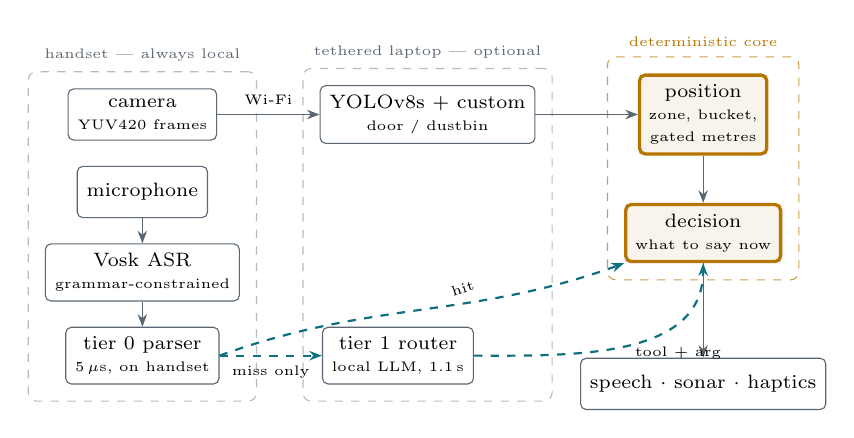
\begin{tikzpicture}[
  font=\scriptsize,
  box/.style={draw=slate, fill=white, rounded corners=2pt, align=center,
              inner sep=3.4pt, minimum height=6.5mm},
  core/.style={box, draw=amber, very thick, fill=amber!8},
  grp/.style={draw=slate!45, dashed, rounded corners=3pt, inner sep=6pt},
  ar/.style={-{Stealth[length=1.6mm]}, draw=slate},
  dar/.style={-{Stealth[length=1.6mm]}, draw=teal, dashed, thick},
  node distance=3.2mm]

\node[box] (cam) {camera\\{\tiny YUV420 frames}};
\node[box, below=of cam] (mic) {microphone};
\node[box, below=of mic] (asr) {Vosk ASR\\{\tiny grammar-constrained}};
\node[box, below=of asr] (t0) {tier 0 parser\\{\tiny 5\,$\mu$s, on handset}};

\node[box, right=13mm of cam] (det) {YOLOv8s + custom\\{\tiny door / dustbin}};
\node[box, right=13mm of t0] (t1) {tier 1 router\\{\tiny local LLM, 1.1\,s}};

\node[core, right=13mm of det] (pos) {position\\{\tiny zone, bucket,}\\{\tiny gated metres}};
\node[core, below=6mm of pos] (dec) {decision\\{\tiny what to say now}};
\node[box, below=12mm of dec] (out) {speech $\cdot$ sonar $\cdot$ haptics};

\begin{scope}[on background layer]
  \node[grp, fit=(cam)(mic)(asr)(t0), label={[font=\tiny,slate]above:handset --- always local}] {};
  \node[grp, fit=(det)(t1), label={[font=\tiny,slate]above:tethered laptop --- optional}] {};
  \node[grp, draw=amber!70, fit=(pos)(dec),
        label={[font=\tiny,amber]above:deterministic core}] {};
\end{scope}

\draw[ar] (cam) -- node[above,font=\tiny]{Wi-Fi} (det);
\draw[ar] (det) -- (pos);
\draw[ar] (pos) -- (dec);
\draw[ar] (dec) -- (out);
\draw[ar] (mic) -- (asr);
\draw[ar] (asr) -- (t0);
\draw[dar] (t0) -- node[below,font=\tiny]{miss only} (t1);
\draw[dar] (t0.east) to[out=20,in=200] node[pos=.62,above,font=\tiny,rotate=18]{hit} (dec.south west);
\draw[dar] (t1.east) to[out=0,in=-90] node[right,font=\tiny,yshift=-1mm]{tool + arg} (dec.south);
\end{tikzpicture}
\caption{The two dashed teal arrows into the deterministic core are the whole
safety argument: the router may point at a capability, but it may not speak
through one. Tier 0 runs on the handset, so every trained phrase still works
with the laptop switched off.}
\Description{Block diagram showing camera and microphone on the handset, a
tethered laptop running detection and the language-model router, and a
deterministic core that produces all spoken guidance.}
\label{fig:system}
\end{figure}

%% ======================================================================
\section{Five ways to decline}
\label{sec:mech}

\textbf{Perception: reliability-gated metric distance.} Distance comes from a
pinhole model, $d = h_{\text{real}} \cdot F / h_{\text{box}}$, and is spoken as
``about $N$ metres'' only if three gates pass: the box does not touch a frame
edge, the class name clears a confidence threshold, and the object is not
already close. The edge-clip gate matters most: a truncated box reads
\emph{falsely far}, so the error points in the dangerous direction, precisely
for the nearest and largest objects. When any gate fails the system speaks the
ordinal bucket instead.

\textbf{Planning: openness-thresholded path advice.} Each of left/ahead/right is
scored by the proximity rank of its \emph{closest} obstacle rather than by summed
occupied area; the naive metric lets a far bulky object outrank a near small
hazard and steers the user into it. Doorways are excluded from obstacle mass. If
even the emptiest third holds a close obstacle, the system refuses to name a
least-bad direction and says ``Stop, no clear path''.

\textbf{Transport: absence is not a negative.} A failed frame returns
\texttt{null}, never an empty list. An empty list means a \emph{verified-clear}
scene, and acting on it silences the sonar, resets escalation state, and makes
Find report ``not visible'' for an object that may be directly ahead. On no-data
the engine pauses guidance and says so.

\textbf{Attention: proximity-gated warnings with a pull counterpart.} Added
after the first field walk, where the verdict was ``it keeps saying all the
objects, it's too much of a cluster''. Continuous warnings now fire only at
close range or nearer; everything removed from the push channel is reachable by
asking (\tool{check}: ``is there anything in front of me?''), answered by the
same ordinal core, in tier 0, with no model and no network. An unheeded warning
has negative value: it spent attention and delivered nothing.

\textbf{Dialogue: routing abstention.} Unknown tool, unknown object class,
missing argument, prose instead of JSON, timeout or any exception all become
abstention, and the clarifying question is selected from a fixed table by key
rather than written by the model.

%% ======================================================================
\section{The agent layer}

BlindAssist's offline recogniser is grammar-constrained: only phrases in an
explicit list can be transcribed \emph{at all}, so free speech is not
mis-parsed---it is never heard. A trigger word therefore opens a dictation
window whose transcript goes first to the deterministic parser and only then, on
a miss, to the router (Figure~\ref{fig:router}).

\textbf{The authority boundary.} The model receives the tool registry, the class
enumeration, a deterministic state block (visible classes with zone, proximity
and count; mode; last announcement; object memory) and the utterance, and must
return JSON. Everything after that treats its output as untrusted input.
Multi-turn references such as ``is it still there'' therefore resolve against
the detector's own output, never against a description: perception never
re-enters the model.

\textbf{Where the boundary moved.} The system as first built enforced the
stronger rule---\emph{no spoken token whatsoever} originated in the model. After
the first field walk the developer-user asked for conversation: the ability to
ask a question in their own words and be answered rather than routed. We granted
exactly that. A reply travels in a separate channel that the executor cannot
route through any capability; it is grounded in the same state block,
length-capped and truncated at a sentence; loose prose emitted where a tool call
belongs is still discarded; and one flag restores the absolute rule for the
ablation. The honest formulation of C2 is therefore ``no \emph{guidance} token
originates in the model'', which is weaker than where we started, and we report
it as weakened.

\textbf{Tiering across a network boundary.} On the handset the two tiers fall on
opposite sides of a Wi-Fi link. The client re-validates the server's reply
against the same closed registry before executing, so the containment guarantee
does not rest on trusting the transport, and a reply containing one unusable
action is discarded whole---executing the half that happened to parse is itself
an unverified action.

\begin{figure}[t]
\centering
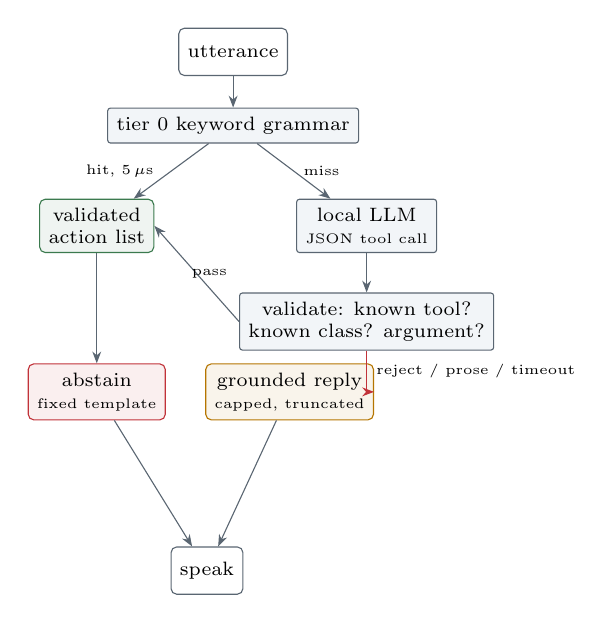
\begin{tikzpicture}[
  font=\scriptsize,
  b/.style={draw=slate, fill=white, rounded corners=2pt, align=center,
            inner sep=3.2pt, minimum height=6mm},
  d/.style={draw=slate, fill=panel, align=center, inner sep=3.2pt,
            rounded corners=1pt},
  ok/.style={b, draw=moss, fill=moss!8},
  no/.style={b, draw=rose, fill=rose!8},
  ar/.style={-{Stealth[length=1.5mm]}, draw=slate},
  node distance=4mm]

\node[b] (u) {utterance};
\node[d, below=of u] (t0) {tier 0 keyword grammar};
\node[ok, below left=7mm and -6mm of t0] (act) {validated\\action list};
\node[d, below right=7mm and -8mm of t0] (llm) {local LLM\\{\tiny JSON tool call}};
\node[d, below=5mm of llm] (val) {validate: known tool?\\known class? argument?};
\node[no, below=14mm of act] (ab) {abstain\\{\tiny fixed template}};
\node[b, draw=amber, fill=amber!8, right=5mm of ab] (say) {grounded reply\\{\tiny capped, truncated}};
\node[b, below=16mm of ab, xshift=14mm] (sp) {speak};

\draw[ar] (u) -- (t0);
\draw[ar] (t0) -- node[left,font=\tiny,xshift=-1mm]{hit, 5\,$\mu$s} (act);
\draw[ar] (t0) -- node[right,font=\tiny]{miss} (llm);
\draw[ar] (llm) -- (val);
\draw[ar] (val.west) -- node[above,font=\tiny,pos=.35]{pass} (act.east);
\draw[ar, draw=rose] (val.south) |- node[right,font=\tiny,pos=.25]{reject / prose / timeout} (say.east);
\draw[ar] (act) -- (ab.north);
\draw[ar] (ab) -- (sp);
\draw[ar] (say) -- (sp);
\end{tikzpicture}
\caption{Two-tier routing. Every path except the amber reply channel produces
text written by deterministic code or by a fixed template.}
\Description{Flow diagram of the two-tier router, showing a keyword tier, a
language-model tier, a validation step, an abstention branch and a separate
grounded-reply branch.}
\label{fig:router}
\end{figure}

%% ======================================================================
\section{Evaluation}

The protocol and a set of 200 labelled utterances were frozen and committed
\emph{before} the router was implemented, so the router could not be tuned
against its own test set. Categories: \emph{canonical} (40, phrasings the
grammar covers), \emph{paraphrase} (70), \emph{multi-intent} (20),
\emph{out-of-scope} (40, gold label: abstain) and \emph{ambiguous} (30, gold
depends on a state block encoded in the record). Configurations: keyword-only,
LLM-only, and two-tier. Routing accuracy is exact match on the ordered action
list. The \emph{over-trigger rate} is the fraction of out-of-scope utterances
answered with any action, and is the safety metric of this layer. The
fabrication check verifies that every executed spoken string is a member of the
set the deterministic core could produce for that record, plus the fixed
templates; the harness fails loudly otherwise.

Model: \tool{llama3.2:3b} under Ollama on the tether laptop.

%% ======================================================================
\section{Results}

\begin{figure}[t]
\centering
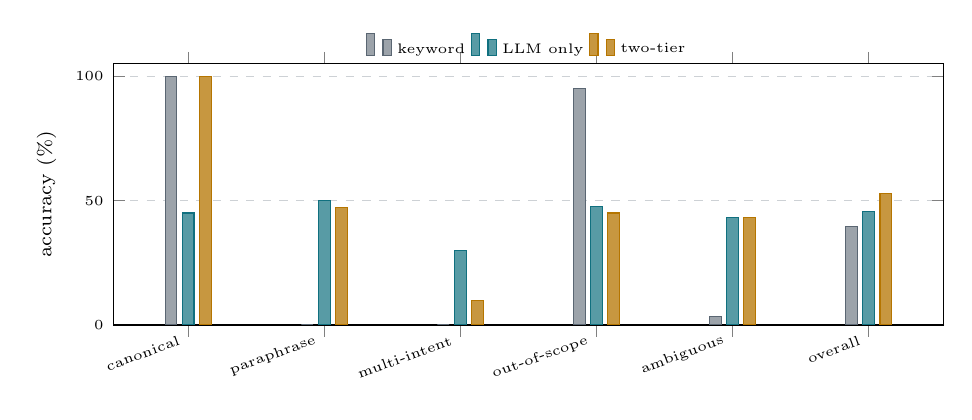
\begin{tikzpicture}
\begin{axis}[
  width=\columnwidth, height=4.9cm,
  ybar, bar width=4.2pt,
  ymin=0, ymax=105,
  ylabel={accuracy (\%)},
  ylabel style={font=\scriptsize},
  symbolic x coords={canonical, paraphrase, multi-intent, out-of-scope, ambiguous, overall},
  xtick=data,
  x tick label style={font=\tiny, rotate=20, anchor=east},
  y tick label style={font=\tiny},
  ymajorgrids, grid style={dashed, slate!30},
  legend style={font=\tiny, at={(0.5,1.14)}, anchor=north, legend columns=3,
                draw=none, fill=none},
  enlarge x limits=0.11,
]
\addplot[fill=slate!60, draw=slate] coordinates
  {(canonical,100) (paraphrase,0) (multi-intent,0) (out-of-scope,95) (ambiguous,3.3) (overall,39.5)};
\addplot[fill=teal!70, draw=teal] coordinates
  {(canonical,45) (paraphrase,50) (multi-intent,30) (out-of-scope,47.5) (ambiguous,43.3) (overall,45.5)};
\addplot[fill=amber!75, draw=amber] coordinates
  {(canonical,100) (paraphrase,47.1) (multi-intent,10) (out-of-scope,45) (ambiguous,43.3) (overall,53)};
\legend{keyword, LLM only, two-tier}
\end{axis}
\end{tikzpicture}
\caption{Routing accuracy by category, $n=200$. For out-of-scope, ``accuracy''
means correctly abstaining. The keyword bars at zero are not degradation but
absence: a grammar cannot hear what is not in its grammar.}
\Description{Grouped bar chart of routing accuracy for three configurations
across five utterance categories and an overall column.}
\label{fig:t3}
\end{figure}

\begin{table}[t]
\caption{Routing accuracy (T3). Wilson 95\% CIs on the overall row: keyword
33.0--46.4, LLM-only 38.7--52.4, two-tier 46.1--59.8.}
\label{tab:t3}
\small
\begin{tabular}{lrrrr}
\toprule
Category & $n$ & keyword & LLM-only & two-tier \\
\midrule
canonical     & 40  & \textbf{100.0} & 45.0 & \textbf{100.0} \\
paraphrase    & 70  & 0.0   & \textbf{50.0} & 47.1 \\
multi-intent  & 20  & 0.0   & \textbf{30.0} & 10.0 \\
out-of-scope  & 40  & \textbf{95.0} & 47.5 & 45.0 \\
ambiguous     & 30  & 3.3   & \textbf{43.3} & \textbf{43.3} \\
\midrule
overall       & 200 & 39.5  & 45.5 & \textbf{53.0} \\
\bottomrule
\end{tabular}
\end{table}

Three things in Table~\ref{tab:t3} matter more than the overall column.

\textbf{The baseline's shape is the motivation stated as data.} It is perfect on
the phrasings it was designed for and zero on paraphrase and multi-intent.

\textbf{Tiering strictly dominates LLM-only.} LLM-only loses 55\% of the
canonical category: the model mis-routes utterances the keyword parser gets
right by construction, usually by substituting a plausible neighbour
(\tool{describe} for \tool{count}, \tool{walk} for \tool{zones}). Two-tier keeps
100\% there because those utterances never reach the model, and still collects
most of the paraphrase gain. The deterministic tier is not a latency
optimisation with an accuracy cost; it is more accurate \emph{and} faster on the
traffic it covers.

\textbf{The abstention collapse is the headline, and it is negative.} The
keyword baseline abstains on 95\% of out-of-scope input for free---an unmatched
utterance returns nothing. Both language-model configurations spend nearly all
of it (Table~\ref{tab:t5}): a 3B model choosing among fourteen tools nearly
always finds one it likes. ``Call my mum'' becomes \tool{read}; ``what time is
it'' becomes \tool{clock}; ``take a photo'' becomes \tool{walk}. We report this
unmitigated because the protocol was frozen before the router existed and tuning
the prompt against this set is what the freeze forbids.

\begin{table}[t]
\caption{Out-of-scope behaviour (T5), $n=40$, and routing latency (T4).}
\label{tab:t5}
\small
\begin{tabular}{lrrr}
\toprule
 & keyword & LLM-only & two-tier \\
\midrule
abstained            & 38 & 19 & 18 \\
answered anyway      & 2  & 21 & 22 \\
over-trigger rate    & \textbf{5.0\%} & 52.5\% & 55.0\% \\
\midrule
tier-0 hit           & 5\,$\mu$s & --- & 5\,$\mu$s \\
tier-1 hit, p50      & --- & 1992\,ms & \textbf{1141\,ms} \\
tier-1 hit, p95      & --- & 3110\,ms & \textbf{2141\,ms} \\
traffic on tier 0    & 30.0\% & 0\% & 30.0\% \\
\bottomrule
\end{tabular}
\end{table}

Both keyword over-triggers are substring collisions: ``read my email'' contains
\emph{read}; ``how do i get to the bus stop'' contains \emph{stop}. They are the
price of matching on keywords, and they are exactly the errors a router with
sentence-level context should remove---it does not, because tier 0 claims them
before the model is consulted. That is the cost side of C3 stated plainly.

Two-tier's tier-1 median is \emph{lower} than LLM-only's because the utterances
that reach the model are the harder, longer ones only. Tier 1 is usable for
on-demand questions and unusable inside a continuous guidance loop; every
capability here is on-demand, which is a fact about this system rather than a
general result.

\begin{figure}[t]
\centering
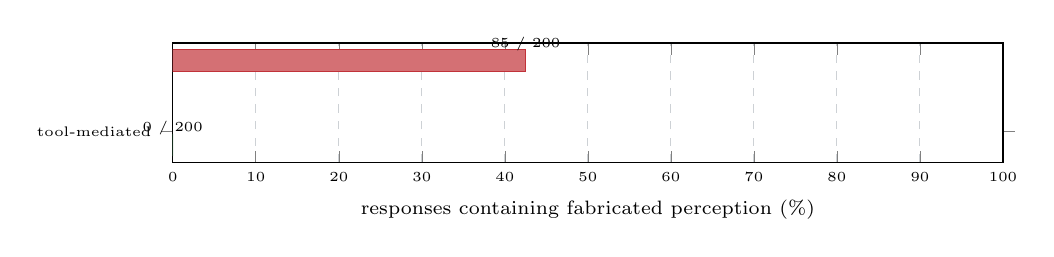
\begin{tikzpicture}
\begin{axis}[
  width=\columnwidth, height=3.1cm,
  xbar, bar width=8pt,
  xmin=0, xmax=100,
  xlabel={responses containing fabricated perception (\%)},
  xlabel style={font=\scriptsize},
  symbolic y coords={tool-mediated, free text},
  ytick=data,
  y tick label style={font=\tiny},
  x tick label style={font=\tiny},
  xmajorgrids, grid style={dashed, slate!30},
  nodes near coords, nodes near coords style={font=\tiny},
  point meta=explicit symbolic,
  enlarge y limits=0.55,
]
\addplot[fill=moss!70, draw=moss] coordinates {(0,tool-mediated) [0 / 200]};
\addplot[fill=rose!70, draw=rose] coordinates {(42.5,free text) [85 / 200]};
\end{axis}
\end{tikzpicture}
\caption{The same model, the same deterministic state block. Asked to
\emph{choose a tool}, it fabricated nothing in any configuration; asked to
\emph{answer}, it fabricated in 42.5\% of responses. The zero is by
construction, not by tuning; the 42.5\% is a keyword-based lower bound counting
invented objects only.}
\Description{Bar chart contrasting zero fabricated responses under tool
mediation with 85 of 200 under free-text answering.}
\label{fig:t6}
\end{figure}

Figure~\ref{fig:t6} is the clearest result in the paper, and the character of
the inventions is worse than the rate suggests. Asked to ``find bottle'' with a
state block listing no bottle, the model replied:

\begin{quote}\itshape
``i'm walking in front of you, my cane tapping on the ground. i've stopped about
6 feet away from your right side. there's a small\ldots''
\end{quote}

It invents an object, a distance in feet, a bearing, and a first-person
travelling companion with a cane. For a sighted user this is a curiosity to
dismiss. For the user this system is built for it arrives in the same voice, at
the same volume, with the same confidence as a real detection.

\textbf{A capability added after the freeze.} The \tool{check} capability was
implemented after the set was committed. Two records are affected and neither
was re-labelled: one paraphrase whose gold we consider superseded, and one
ambiguous record whose failure mode changed from silent abstention to a
confident answer to a different question---strictly worse, and the predictable
cost of widening a keyword grammar. A third instance was caught by the frozen
out-of-scope category before any user met it: the first implementation treated
any ``left'' as a direction, so ``how much battery is left'' routed to a scene
query, raising over-trigger to 7.5\%. The rule now requires a positional lead-in
for that ambiguous pair.

%% ======================================================================
\section{Discussion and limitations}

\textbf{No blind participants.} The system has been field-walked by a single
sighted developer. Every claim here about what is \emph{safer} is a design
argument supported by mechanism and by deterministic tests, not by user data. A
study with blind participants is the necessary next step and specifically the
one that could falsify the premise: users may prefer a guessed answer to an
abstention.

\textbf{Over-triggering is measured, not solved.} 55\% is the largest open
problem this evaluation exposes. Rejection examples in the prompt, a second-pass
scope classifier, and a model-confidence gate are all available; none is
evaluated, because each would be tuning against a frozen set. A held-out set
comes first.

\textbf{One model, one machine.} A second arm with a reasoning model
(\tool{qwen3:4b}) returned no parseable tool call on 102 of 140 tier-1 calls at
6--8\,s each, so tier 1 contributed nothing and the run scored exactly the
keyword baseline. The validation boundary degraded to fewer capabilities rather
than to wrong ones, which is the designed behaviour, but the comparison is not
informative about model size until thinking output is disabled.

\textbf{The clock mapping is camera-frame, not O\&M.} Frame width spans 10--2
o'clock over roughly a 60$^\circ$ field of view, so ``2 o'clock'' means the right
frame edge, not the 90$^\circ$ a trained traveller would turn.

\textbf{Distance is coarse and the fabrication detector is crude.} Roughly
$\pm$30--40\% at 5\,m with an uncalibrated focal constant; the gating argument
concerns \emph{when} to speak a number, not how good it is. The detector flags
invented objects only, missing invented distances and bearings---several of
which appear in the samples it did flag. Reported as a lower bound.

\textbf{Chat replies are counted, not judged.} They are excluded from the
fabrication metric by definition and listed for inspection, but we do not
measure whether they are correct or well-calibrated.

%% ======================================================================
\section{Conclusion}

For users who cannot audit what a system tells them, abstention is not an error
path---it is a feature that must be designed, implemented and measured at every
layer where the system can be wrong. We showed five such designs in a working
offline assistive system, each with criteria specific to its layer's failure
mode, and extended the pattern to a voice agent whose language model may choose
what the system does and never what it says about the world. The interesting
claim is not that tool mediation prevents hallucination---it plainly does---but
that the same principle that motivates it also explains a distance gate, a path
threshold, a null-versus-empty distinction, and a warning-rate ceiling, three
layers away.

\begin{table}[t]
\caption{The capability registry. One declarative table drives the recogniser's
phrase list, the model's tool schema, the executor, and a manifest both language
test suites assert against.}
\label{tab:registry}
\small
\begin{tabular}{llp{3.1cm}}
\toprule
Tool & Argument & Backed by \\
\midrule
\tool{walk}     & ---              & engine mode \\
\tool{find}     & class, required  & \tool{find\_message} \\
\tool{describe} & ---              & \tool{summarize\_scene} \\
\tool{count}    & class, required  & \tool{count\_message} \\
\tool{recall}   & class, required  & object memory \\
\tool{path}     & ---              & \tool{clear\_path} \\
\tool{check}    & direction, req.  & \tool{check\_direction} \\
\tool{read}     & ---              & on-device OCR \\
\tool{clock} / \tool{zones} & ---  & bearing style \\
\tool{sonar}    & on/off           & sonar controller \\
\tool{mute}     & on/off, required & speech controller \\
\tool{stop} / \tool{repeat} & ---  & speech controller \\
\tool{abstain}  & template key     & fixed template table \\
\bottomrule
\end{tabular}
\end{table}

\end{document}
